\documentclass[11pt]{article}

\usepackage[margin=1in]{geometry}
\usepackage{amsmath,amssymb,amsthm}
\usepackage{mathtools}
\usepackage{bm}
\usepackage{graphicx}
\usepackage{booktabs}
\usepackage{enumitem}
\usepackage{hyperref}
\usepackage{microtype}
\usepackage{titlesec}
\usepackage{fancyhdr}
\usepackage{caption}

\hypersetup{colorlinks=true,linkcolor=black,urlcolor=blue,citecolor=blue}
\setcounter{tocdepth}{2}
\numberwithin{equation}{section}

\titleformat{\section}{\large\bfseries}{\thesection.}{0.6em}{}
\titleformat{\subsection}{\normalsize\bfseries}{\thesubsection}{0.5em}{}
\titleformat{\subsubsection}{\normalsize\itshape}{\thesubsubsection}{0.5em}{}

\pagestyle{fancy}
\fancyhf{}
\fancyhead[L]{\small Deep learning theory}
\fancyhead[R]{}
\fancyfoot[C]{\thepage}
\renewcommand{\headrulewidth}{0.3pt}

\graphicspath{{figures/}}
\captionsetup{font=small,skip=6pt}

\theoremstyle{definition}
\newtheorem{definition}{Definition}[section]
\newtheorem{remark}{Remark}[section]
\newtheorem{exercise}{Exercise}[section]

\newenvironment{solution}{%
  \par\medskip\noindent\textit{Solution.}\enspace
}{\par\medskip}

\newcommand{\ansbox}[1]{%
  \par\smallskip
  \noindent
  \fbox{\parbox{\dimexpr\linewidth-2\fboxsep-2\fboxrule\relax}{\textbf{Answer.} #1}}%
  \par\smallskip
}

\theoremstyle{plain}
\newtheorem{proposition}{Proposition}[section]
\newtheorem{lemma}{Lemma}[section]
\newtheorem{theorem}{Theorem}[section]
\newtheorem{corollary}{Corollary}[section]

\newcommand{\R}{\mathbb{R}}
\newcommand{\E}{\mathbb{E}}
\newcommand{\dd}{\mathrm{d}}
\newcommand{\id}{\mathbf{1}}
\newcommand{\one}{\mathbf{1}}
\newcommand{\h}{\mathbf{h}}
\newcommand{\x}{\mathbf{x}}
\newcommand{\w}{\mathbf{w}}
\newcommand{\W}{\mathbf{W}}
\newcommand{\ph}{\varphi}
\newcommand{\Th}{\Theta}
\newcommand{\ntk}{\Theta}
\newcommand{\loss}{\mathcal{L}}
\newcommand{\hyp}{\mathcal{H}}
\newcommand{\data}{\mathcal{D}}
\newcommand{\on}[1]{O_{N}(#1)}
\newcommand{\ON}[1]{O_{N}(#1)}
\newcommand{\pd}[2]{\frac{\partial #1}{\partial #2}}
\newcommand{\td}[2]{\frac{\mathrm{d} #1}{\mathrm{d} #2}}
\newcommand{\inner}[2]{\left\langle #1,#2\right\rangle}
\newcommand{\norm}[1]{\left\|#1\right\|}
\newcommand{\diag}{\mathrm{diag}}
\newcommand{\tr}{\mathrm{tr}}
\newcommand{\ind}{\mathbf{1}}
\renewcommand{\vec}[1]{\mathbf{#1}}

\DeclareMathOperator*{\argmin}{arg\,min}
\DeclareMathOperator{\Var}{Var}
\DeclareMathOperator{\Cov}{Cov}
\newcommand{\ie}{\textit{i.e.}}
\newcommand{\eg}{\textit{e.g.}}


\title{Deep Learning Theory\\[0.4em]
\large Kernels, infinite width, and effective theory}
\author{}
\date{}

\begin{document}
\maketitle
\vspace{-1.4em}
\begin{center}
\small Notation follows Pehlevan and Bordelon~\cite{pehlevan2023infinite}
and Roberts, Yaida, and Hanin~\cite{roberts2022pdlt}.
\end{center}

\tableofcontents
\newpage

\section{Setting}

A feedforward MLP of depth $L$ and width $N$ maps $x\in\R^{D}$ to a scalar by
\begin{align}
  h^{(0)} &= x, \nonumber\\
  h^{(\ell+1)} &= N^{-a_{\ell+1}} W^{(\ell+1)}\,\ph\!\big(h^{(\ell)}\big),
  \qquad \ell=0,\ldots,L-2, \nonumber\\
  f &= \gamma^{-1} N^{-a_L}\, w\cdot\ph\!\big(h^{(L-1)}\big).
  \label{eq:mlp-schema}
\end{align}
The activation $\ph$ is applied elementwise. Weights are drawn $W^{(\ell)}_{ij}\sim\mathcal{N}(0,N^{-b_\ell})$, and the training set is $\data=\{(x_\mu,y_\mu)\}_{\mu=1}^{P}$. Two kernels appear throughout:
\begin{equation}
  \Phi^{(\ell)}_{\mu\nu}
  \equiv
  N^{-1}\,\ph\!\big(h^{(\ell)}_\mu\big)\cdot\ph\!\big(h^{(\ell)}_\nu\big),
  \qquad
  K_{\mu\nu}(t)
  \equiv
  \partial_\theta f(x_\mu;t)\cdot\partial_\theta f(x_\nu;t).
  \label{eq:two-kernels}
\end{equation}
The first is the \emph{feature kernel} of layer $\ell$. The second is the \emph{neural tangent kernel}. In the limits treated here both concentrate, and the $O(N)$ weights are replaced by $O(P^2)$ kernel entries.

The questions are: which functions~\eqref{eq:mlp-schema} can represent; how $f(\,\cdot\,;\theta(t))$ moves under gradient flow; and what the population risk is after training. The answers depend on how $(a_\ell,b_\ell,\gamma)$ scale with $N$, and on the ratio $L/N$.

\section{Supervised learning}
\label{sec:supervised}

Inputs $x\in\mathcal{X}\subset\R^{D}$ and labels $y\in\mathcal{Y}\subset\R$ are jointly distributed as $P(x,y)$. A predictor $h$ is taken from a hypothesis class $\hyp$. For a neural net, $\hyp$ is the image of $\theta\mapsto f(\,\cdot\,;\theta)$.

A loss $\ell:\mathcal{Y}\times\mathcal{Y}\to\R_{\ge 0}$ compares prediction and label. Two standard choices:
\begin{equation}
  \ell_{\mathrm{sq}}(h(x),y)=\tfrac12\bigl(h(x)-y\bigr)^2,
  \qquad
  \ell_{01}(h(x),y)=\ind\bigl[h(x)\neq y\bigr].
  \label{eq:losses}
\end{equation}

\begin{definition}[Population and empirical risk]
\begin{equation}
  R(h)\equiv \E_{(x,y)\sim P}\bigl[\ell(h(x),y)\bigr],
  \qquad
  \hat R_{\data}(h)\equiv\frac1P\sum_{\mu=1}^{P}\ell\bigl(h(x_\mu),y_\mu\bigr),
  \label{eq:risks}
\end{equation}
where $\data=\{(x_\mu,y_\mu)\}_{\mu=1}^{P}\sim P^{\otimes P}$.
\end{definition}

The Bayes predictor $h_{\mathrm{Bayes}}=\argmin R(h)$ is over all measurable functions and need not lie in $\hyp$. The best-in-class predictor is $h^\star=\argmin_{h\in\hyp} R(h)$. Training does not see $P$. Empirical risk minimization replaces the population problem by
\begin{equation}
  h_{\data,\mathrm{ERM}}=\argmin_{h\in\hyp}\hat R_{\data}(h).
  \label{eq:erm}
\end{equation}

\begin{lemma}
For any \emph{fixed} $h$, $\E_{\data}[\hat R_{\data}(h)]=R(h)$.
\end{lemma}
\begin{proof}
Linearity of expectation; the $P$ samples are identically distributed.
\end{proof}
Once $h$ depends on $\data$, the identity fails: $\E_{\data}[\hat R_{\data}(h_{\data})]$ is optimistically biased. The generalization gap is
\begin{equation}
  \Delta_{\mathrm{gen}}(h_{\data})\equiv R(h_{\data})-\hat R_{\data}(h_{\data}).
  \label{eq:gen-gap}
\end{equation}
\emph{Generalization error} will mean $R(h_{\data})$ itself.

Write $h(x)=f(x;\theta)$. Square loss on $\data$ is
\begin{equation}
  \loss(\theta)
  \equiv
  \frac1{2P}\sum_{\mu=1}^{P}\bigl(f(x_\mu;\theta)-y_\mu\bigr)^2,
  \label{eq:sq-loss}
\end{equation}
so $\partial\loss/\partial f_\mu=(f_\mu-y_\mu)/P$. Gradient descent and its gradient-flow limit are
\begin{equation}
  \theta_{t+1}=\theta_t-\eta\,\nabla_\theta\loss(\theta_t),
  \qquad
  \td{\theta}{t}=-\eta\,\nabla_\theta\loss(\theta).
  \label{eq:gd-gf}
\end{equation}

\begin{exercise}
Verify $\E_{\data}[\hat R_{\data}(h)]=R(h)$ from~\eqref{eq:risks}. Where does the argument use that $h$ does not depend on $\data$?
\end{exercise}

\section{Feature spaces and kernel machines}
\label{sec:kernels}

\subsection{Maximum-margin hyperplanes}

A linear classifier $h(x)=\mathrm{sign}(w\cdot x+b)$ on a linearly separable sample admits many separating hyperplanes. The \emph{margin} of $(w,b)$ is the distance to the nearest training point,
\begin{equation}
  \delta^\star=\min_{\mu\in[P]}\frac{\lvert w\cdot x_\mu+b\rvert}{\|w\|}.
  \label{eq:margin}
\end{equation}
The scale $(w,b)\sim(\alpha w,\alpha b)$ is redundant. Canonicalize by $\min_\mu\lvert w\cdot x_\mu+b\rvert=1$, so that $\delta^\star=1/\|w\|$. Maximizing the margin is then
\begin{equation}
  \min_{w,b}\ \tfrac12\|w\|^2
  \qquad\text{subject to}\qquad
  y_\mu(w\cdot x_\mu+b)\ge 1
  \quad\forall\mu.
  \label{eq:hard-margin}
\end{equation}

The Lagrangian is
\begin{equation}
  L(w,b,\alpha)
  =\tfrac12\|w\|^2
  -\sum_{\mu=1}^{P}\alpha_\mu\bigl(y_\mu(w\cdot x_\mu+b)-1\bigr),
  \qquad \alpha_\mu\ge 0.
  \label{eq:lagrange}
\end{equation}
Stationarity in $(w,b)$ gives the KKT conditions
\begin{equation}
  w=\sum_{\mu=1}^{P}\alpha_\mu y_\mu x_\mu,
  \qquad
  \sum_{\mu=1}^{P}\alpha_\mu y_\mu=0,
  \qquad
  \alpha_\mu\bigl(y_\mu(w\cdot x_\mu+b)-1\bigr)=0.
  \label{eq:kkt}
\end{equation}
Complementary slackness forces $\alpha_\mu=0$ unless the constraint is tight. Those points are the \emph{support vectors}; they alone determine $w$. Substituting~\eqref{eq:kkt} back into $L$ produces the dual
\begin{equation}
  \max_{\alpha\ge 0}\
  \sum_{\mu}\alpha_\mu
  -\tfrac12\sum_{\mu\nu}\alpha_\mu\alpha_\nu y_\mu y_\nu\, x_\mu\cdot x_\nu
  \qquad\text{s.t.}\qquad
  \sum_{\mu}\alpha_\mu y_\mu=0.
  \label{eq:svm-dual}
\end{equation}
The data enter only through the Gram matrix $G_{\mu\nu}=x_\mu\cdot x_\nu$. The classifier itself is
\begin{equation}
  h(x)=\mathrm{sign}\!\left(\sum_{\mu}\alpha_\mu y_\mu\, x\cdot x_\mu+b\right).
  \label{eq:svm-pred}
\end{equation}

\begin{figure}[ht]
\centering
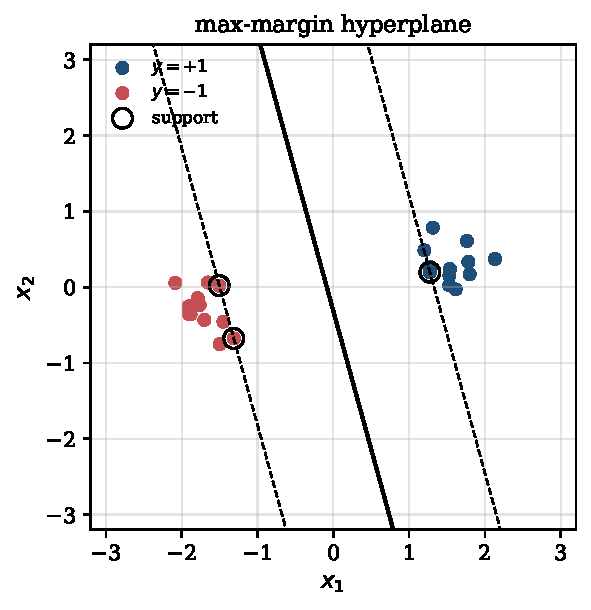
\includegraphics[width=0.62\textwidth]{fig06_margin.pdf}
\caption{Hard-margin SVM in $\R^2$. Solid line: $w\cdot x+b=0$. Dashed: $w\cdot x+b=\pm 1$. Circled points are the support vectors.}
\label{fig:margin}
\end{figure}

\subsection{The kernel trick}

If $\{(x_\mu,y_\mu)\}$ is not linearly separable in $\R^{D}$, lift through a feature map $\Phi:\R^{D}\to\R^{M}$, $M\ge D$, and run the same SVM on $\Phi(x)$. The dual~\eqref{eq:svm-dual} and the predictor~\eqref{eq:svm-pred} depend on $\Phi$ only through
\begin{equation}
  K(x,x')\equiv\Phi(x)\cdot\Phi(x').
  \label{eq:kernel-def}
\end{equation}
One never instantiates $\Phi$. It is enough that $K$ be a symmetric positive-definite kernel (Mercer's theorem): there exist $\lambda_k\ge 0$ and orthonormal $\psi_k$ on $L^2(P_x)$ with
\begin{equation}
  K(x,x')=\sum_{k}\lambda_k\,\psi_k(x)\psi_k(x').
  \label{eq:mercer-kernel}
\end{equation}
The associated feature map is $\Phi(x)_k=\sqrt{\lambda_k}\,\psi_k(x)$, possibly infinite-dimensional.

\begin{theorem}[Representer]
Any minimizer of $\hat R_{\data}(h)+\lambda\|h\|_{\mathcal{H}_K}^2$ over the RKHS of $K$ is of the form
$h(\,\cdot\,)=\sum_{\mu=1}^{P}c_\mu K(x_\mu,\,\cdot\,)$.
\end{theorem}
The coefficients $c\in\R^{P}$ are the only degrees of freedom. Kernel ridge with the square loss~\eqref{eq:sq-loss} plus $\tfrac\lambda2\|w\|^2$ is derived in~\S\ref{sec:gen}:
\begin{equation}
  f(x)=k(x)^\top(\hat K+\lambda P I)^{-1} y,
  \qquad
  \hat K_{\mu\nu}=K(x_\mu,x_\nu),\quad
  k(x)_\mu=K(x,x_\mu).
  \label{eq:ridge}
\end{equation}

\subsection{A neural kernel}

A random one-hidden-layer net
\begin{equation}
  f(x)=N^{-1/2}\sum_{i=1}^{N} v_i\,\ph(w_i\cdot x),
  \qquad w_i\sim\mathcal{N}(0,D^{-1}I),\ \ v_i\sim\mathcal{N}(0,1),
  \label{eq:shallow}
\end{equation}
defines, at initialization, the kernel
\begin{equation}
  K_{\mathrm{NNGP}}(x,x')
  =\E_{w,v}\bigl[f(x)f(x')\bigr]
  =\E_{w}\bigl[\ph(w\cdot x)\ph(w\cdot x')\bigr].
  \label{eq:nngp-shallow}
\end{equation}
For $\ph(z)=\max(z,0)$ this is the Cho--Saul kernel. Derive it as follows. Let $w\sim\mathcal{N}(0,I)$, set $u=\hat x\cdot w$ and $u'=\hat x'\cdot w$ with $\hat x=x/\|x\|$, and write $\vartheta=\arccos(\hat x\cdot\hat x')$. Then $(u,u')$ is a standard bivariate Gaussian with correlation $\cos\vartheta$, equivalently the two coordinates of a 2d standard Gaussian $g$ in the plane of $(\hat x,\hat x')$:
\begin{equation}
  u=\rho\cos\phi,\qquad u'=\rho\cos(\phi-\vartheta),\qquad
  g=(\rho\cos\phi,\rho\sin\phi).
\end{equation}
ReLU is supported on $u>0$, $u'>0$, a wedge of opening $\pi-\vartheta$, namely $\phi\in(\vartheta-\pi/2,\pi/2)$. The Gaussian measure on the plane is $e^{-\rho^2/2}\,\rho\,\dd\rho\,\dd\phi/(2\pi)$, so
\begin{equation}
  \E[u_+u'_+]
  =\int_{\vartheta-\pi/2}^{\pi/2}\!\dd\phi
  \int_0^\infty\!\dd\rho\
  \frac{\rho^3 e^{-\rho^2/2}}{2\pi}\,\cos\phi\cos(\phi-\vartheta).
\end{equation}
The radial integral is $\int_0^\infty\rho^3 e^{-\rho^2/2}\,\dd\rho=2$. For the angle, $\cos\phi\cos(\phi-\vartheta)=\tfrac12\bigl(\cos(2\phi-\vartheta)+\cos\vartheta\bigr)$, so
\begin{equation}
  \int_{\vartheta-\pi/2}^{\pi/2}\cos\phi\cos(\phi-\vartheta)\,\dd\phi
  =\Bigl[\tfrac14\sin(2\phi-\vartheta)+\tfrac\phi2\cos\vartheta\Bigr]_{\vartheta-\pi/2}^{\pi/2}
  =\tfrac12\bigl(\sin\vartheta+(\pi-\vartheta)\cos\vartheta\bigr).
\end{equation}
Hence $\E[u_+u'_+]=(2\pi)^{-1}\bigl(\sin\vartheta+(\pi-\vartheta)\cos\vartheta\bigr)$. Scaling back $w\sim\mathcal{N}(0,D^{-1}I)$ multiplies by $\|x\|\|x'\|/D$:
\begin{equation}
  \E\bigl[\ph(w\cdot x)\ph(w\cdot x')\bigr]
  =\frac{\|x\|\|x'\|}{2\pi D}\bigl(\sin\vartheta+(\pi-\vartheta)\cos\vartheta\bigr).
  \label{eq:cho-saul}
\end{equation}
Deeper random nets compose this expectation layer by layer: that is the NNGP recursion below.

\begin{figure}[ht]
\centering
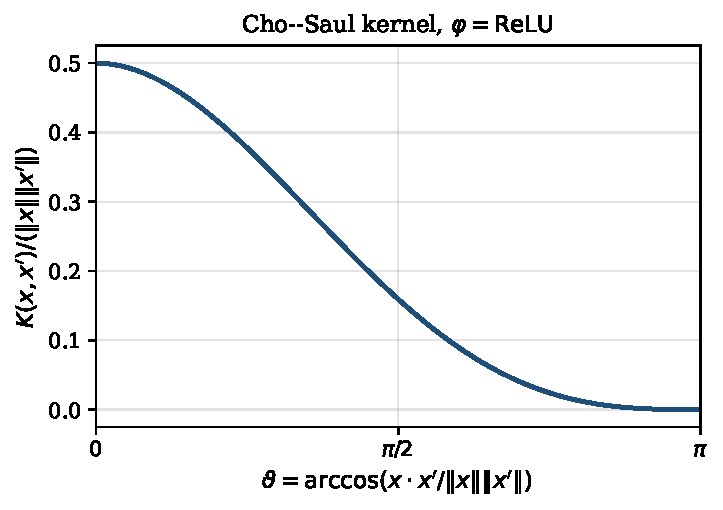
\includegraphics[width=0.72\textwidth]{fig07_chosaul.pdf}
\caption{Unit-variance Cho--Saul factor $\E[u_+u'_+]=(2\pi)^{-1}(\sin\vartheta+(\pi-\vartheta)\cos\vartheta)$ as a function of the angle between $x$ and $x'$.}
\label{fig:chosaul}
\end{figure}

\begin{exercise}
From~\eqref{eq:kkt}, show that if $x_\mu$ is not a support vector then $\alpha_\mu=0$. Conclude that $w$ is a linear combination of the support vectors only.
\end{exercise}
\begin{solution}
Complementary slackness in~\eqref{eq:kkt} is $\alpha_\mu\bigl(y_\mu(w\cdot x_\mu+b)-1\bigr)=0$. If $x_\mu$ is not a support vector the inequality is slack, $y_\mu(w\cdot x_\mu+b)>1$, so the second factor is nonzero and therefore $\alpha_\mu=0$. The stationarity condition $w=\sum_{\nu}\alpha_\nu y_\nu x_\nu$ then retains only those $\nu$ with $\alpha_\nu\neq 0$, i.e.\ the support vectors.
\ansbox{$x_\mu$ not on the margin $\Rightarrow$ $\alpha_\mu=0$, hence $w=\sum_{\mathrm{SV}}\alpha_\nu y_\nu x_\nu$.}
\end{solution}

\section{Training dynamics and the NTK}
\label{sec:ntk}

Let $f(x;\theta)$ be scalar, $f_\mu\equiv f(x_\mu;\theta)$, and $\Delta_\mu\equiv -\partial\ell_\mu/\partial f_\mu$. For~\eqref{eq:sq-loss},
\begin{equation}
  \Delta_\mu=y_\mu-f_\mu.
  \label{eq:delta-sq}
\end{equation}

\subsection{Function-space gradient flow}

Chain rule on~\eqref{eq:gd-gf}:
\begin{equation}
  \td{f(x)}{t}
  =\partial_\theta f(x)\cdot\td{\theta}{t}
  =-\eta\,\partial_\theta f(x)\cdot\nabla_\theta\loss.
  \label{eq:chain}
\end{equation}
The loss gradient is $\nabla_\theta\loss=P^{-1}\sum_{\mu}(\partial\ell_\mu/\partial f_\mu)\,\partial_\theta f_\mu$, so
\begin{equation}
  \partial_t f(x)
  =\frac{\eta}{P}\sum_{\mu=1}^{P}
  \underbrace{\bigl(\partial_\theta f(x)\cdot\partial_\theta f(x_\mu)\bigr)}_{K(x,x_\mu;t)}
  \Delta_\mu.
  \label{eq:fn-ode}
\end{equation}

\begin{definition}[Neural tangent kernel]
\begin{equation}
  K(x,x';t)
  \equiv
  \partial_\theta f(x;\theta(t))\cdot\partial_\theta f(x';\theta(t)).
  \label{eq:ntk-def}
\end{equation}
On the training set, $\hat K_{\mu\nu}(t)\equiv K(x_\mu,x_\nu;t)$ and $k(x;t)_\mu\equiv K(x,x_\mu;t)$.
\end{definition}
$K$ is a Gram matrix of Jacobians, hence positive semidefinite. Equation~\eqref{eq:fn-ode} is exact at any finite width. It is not closed: $K(t)$ depends on $\theta(t)$.

\subsection{Frozen kernel}

Suppose $K(x,x';t)=K(x,x';0)\equiv K(x,x')$. On the training points,
\begin{equation}
  \partial_t F
  =\frac{\eta}{P}\,\hat K\,(y-F),
  \qquad
  F_\mu(t)\equiv f(x_\mu;t).
  \label{eq:train-ode}
\end{equation}
Diagonalize $\hat K=U\Lambda U^\top$, $\Lambda=\mathrm{diag}(\lambda_i)$. In the eigenbasis $F'=U^\top F$, $y'=U^\top y$,
\begin{equation}
  \partial_t F'_i=\frac{\eta\lambda_i}{P}(y'_i-F'_i)
  \quad\Longrightarrow\quad
  F'_i(t)=y'_i+e^{-(\eta\lambda_i/P)t}\bigl(F'_i(0)-y'_i\bigr).
  \label{eq:mode-ode}
\end{equation}
Mode $i$ trains on the timescale $P/(\eta\lambda_i)$.

\begin{figure}[ht]
\centering
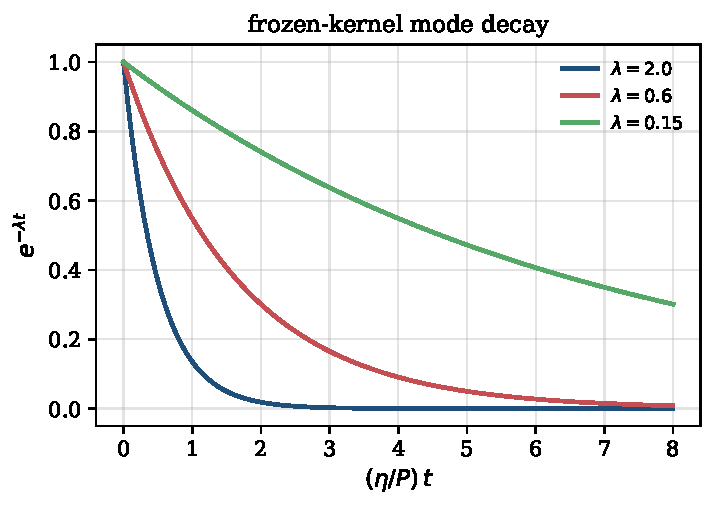
\includegraphics[width=0.72\textwidth]{fig08_modes.pdf}
\caption{Eigenmodes of a frozen kernel. Residual of mode $i$ decays as $e^{-(\eta\lambda_i/P)t}$.}
\label{fig:modes}
\end{figure}

Transforming back,
\begin{equation}
  F(t)
  =y+e^{-(\eta/P)\hat K\, t}\bigl(F(0)-y\bigr)
  =F(0)+\bigl(I-e^{-(\eta/P)\hat K\, t}\bigr)\bigl(y-F(0)\bigr).
  \label{eq:F-sol}
\end{equation}
A test point is slaved to the training residual. Substituting~\eqref{eq:F-sol} into~\eqref{eq:fn-ode},
\begin{equation}
  f(x;t)
  =f(x;0)
  +k(x)^\top\hat K^{-1}
  \bigl(I-e^{-(\eta/P)\hat K\, t}\bigr)
  \bigl(y-F(0)\bigr),
  \label{eq:test-sol}
\end{equation}
with the pseudoinverse if $\hat K$ is singular (the component of $y-F(0)$ in $\ker\hat K$ never trains). As $t\to\infty$ with $f(\,\cdot\,;0)=0$,
\begin{equation}
  f(x;\infty)=k(x)^\top\hat K^{-1} y,
  \label{eq:ridgeless}
\end{equation}
which is~\eqref{eq:ridge} at $\lambda=0$.

\subsection{Linear models}

If $f(x;w)=w\cdot\Phi(x)$ with $\Phi$ fixed, then
\begin{equation}
  \td{w}{t}
  =\frac{\eta}{P}\sum_{\mu}\bigl(y_\mu-w\cdot\Phi(x_\mu)\bigr)\,\Phi(x_\mu),
  \label{eq:lin-gf}
\end{equation}
and
\begin{equation}
  \partial_t f(x)
  =\frac{\eta}{P}\sum_{\mu} K_\Phi(x,x_\mu)\bigl(y_\mu-f(x_\mu)\bigr),
  \qquad
  K_\Phi(x,x')=\Phi(x)\cdot\Phi(x').
  \label{eq:lin-fn}
\end{equation}
The NTK of a linear model \emph{is} $K_\Phi$, and it cannot move. Adding $\tfrac{\lambda}{2}\|w\|^2$ to~\eqref{eq:sq-loss} replaces $\hat K^{-1}$ by $(\hat K+\lambda P I)^{-1}$; see~\S\ref{sec:gen}.

\subsection{Two-layer NTK}

For $f(x)=N^{-1/2}v\cdot\ph(Wx/\sqrt{D})$ the Jacobian splits over $v$ and $W$:
\begin{align}
  \partial_{v_i}f(x) &= N^{-1/2}\ph(h_i(x)), \nonumber\\
  \partial_{W_{ij}}f(x) &= N^{-1/2}D^{-1/2}\,v_i\,\dot\ph(h_i(x))\,x_j,
  \label{eq:two-jac}
\end{align}
with $h(x)=Wx/\sqrt{D}$. Therefore
\begin{equation}
  K(x,x')
  =N^{-1}\,\ph(h(x))\cdot\ph(h(x'))
  +N^{-1}D^{-1}\bigl(v\odot\dot\ph(h(x))\bigr)\cdot\bigl(v\odot\dot\ph(h(x'))\bigr)\,(x\cdot x').
  \label{eq:two-ntk}
\end{equation}
The first term is the feature kernel $\Phi$. The second is the contribution of the first-layer weights. At infinite $N$ both concentrate, and if $v,W$ move by $o_N(1)$ then $K(t)=K(0)$.

\begin{figure}[ht]
\centering
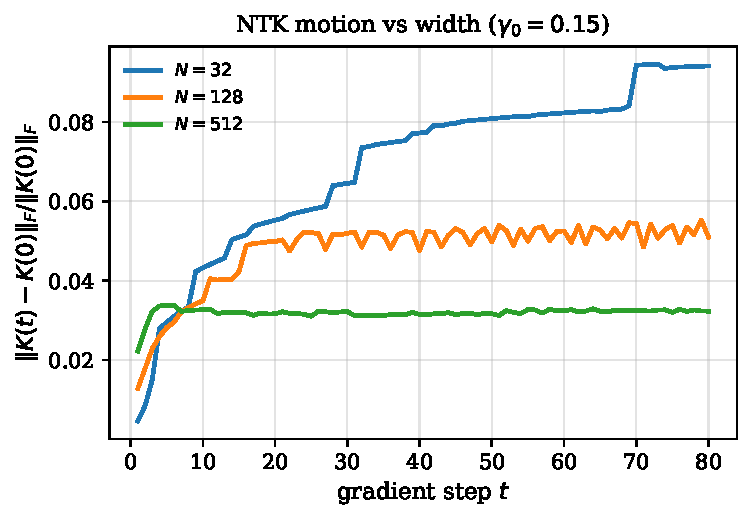
\includegraphics[width=0.72\textwidth]{fig01_ntk_freeze.pdf}
\caption{Two-layer ReLU, $\gamma_0=0.15$, square loss. Relative Frobenius change of the empirical NTK on the training set, for widths $N=32,128,512$.}
\label{fig:ntk-freeze}
\end{figure}

\subsection{Expressivity}

\begin{theorem}[Cybenko, Hornik]
If $\ph$ is continuous, bounded, and nonconstant, then shallow nets $x\mapsto\sum_{i=1}^{N}v_i\ph(w_i\cdot x+b_i)$ are dense in $C([0,1]^D)$ in the uniform norm.
\end{theorem}
Density does not control the number of neurons. For ReLU nets of depth $L$ and width $N$ on $N_0$ inputs, each hidden unit folds the input space along a hyperplane. A lower bound on the number of linear regions is
\begin{equation}
  \Omega\!\left(\left(\frac{N}{N_0}\right)^{(L-1)N_0} N^{N_0}\right).
  \label{eq:regions}
\end{equation}
A matched-parameter shallow net ($L=1$, width $NL$) has only $O\bigl((NL)^{N_0}\bigr)$ regions. Depth buys exponentially many linear pieces per parameter.

\begin{figure}[ht]
\centering
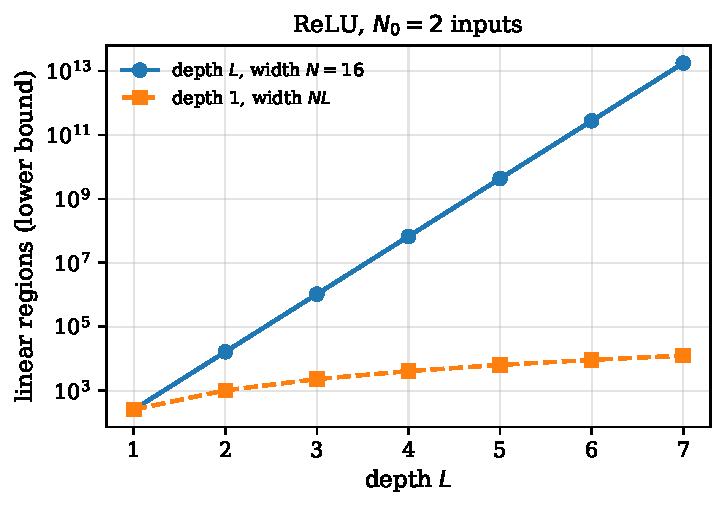
\includegraphics[width=0.72\textwidth]{fig09_regions.pdf}
\caption{Lower bound~\eqref{eq:regions} versus a shallow net with the same number of units $NL$, for $N_0=2$, $N=16$.}
\label{fig:regions}
\end{figure}

\begin{exercise}
Starting from~\eqref{eq:train-ode}, derive~\eqref{eq:F-sol} by expanding $F$ in the eigenbasis of $\hat K$. What is the training time of a mode with kernel eigenvalue $\lambda$?
\end{exercise}
\begin{solution}
Let $\hat K=U\Lambda U^\top$ with $\Lambda=\mathrm{diag}(\lambda_i)$ and set $F'=U^\top F$, $y'=U^\top y$. Substitute into~\eqref{eq:train-ode}:
\[
  \partial_t F'
  =\frac{\eta}{P}\Lambda(y'-F'),
\]
which decouples: $\partial_t F'_i=(\eta\lambda_i/P)(y'_i-F'_i)$. The ODE $\dot u=-a(u-b)$ with $a=\eta\lambda_i/P$ and $b=y'_i$ integrates to
\[
  F'_i(t)=y'_i+e^{-(\eta\lambda_i/P)t}\bigl(F'_i(0)-y'_i\bigr).
\]
In matrix form $F'(t)=y'+e^{-(\eta/P)\Lambda t}(F'(0)-y')$. Multiplying by $U$ and using $U e^{-(\eta/P)\Lambda t}U^\top=e^{-(\eta/P)\hat K t}$ gives~\eqref{eq:F-sol}. Mode $i$ has time constant $P/(\eta\lambda_i)$.
\ansbox{$F(t)=y+e^{-(\eta/P)\hat K t}(F(0)-y)$. Mode with eigenvalue $\lambda$ trains on the timescale $P/(\eta\lambda)$.}
\end{solution}

\section{Lazy versus rich parameterization}
\label{sec:lazy}

Whether $K(t)$ stays at $K(0)$ is a scaling question~\cite{chizat2019lazy,yang2021mup,pehlevan2023infinite}. Write
\begin{align}
  h^{(1)}_\mu &= N^{-a_1} W^{(1)} x_\mu, &
  h^{(\ell+1)}_\mu &= N^{-a_{\ell+1}} W^{(\ell+1)}\ph\!\big(h^{(\ell)}_\mu\big), &
  f_\mu &= \gamma^{-1} N^{-a_L}\, w\cdot\ph\!\big(h^{(L-1)}_\mu\big),
  \label{eq:pb-mlp}
\end{align}
with $W^{(\ell)}_{ij}\sim\mathcal{N}(0,N^{-b_\ell})$ and learning rate
\begin{equation}
  \eta=\eta_0\,\gamma^2 N^{c},
  \qquad
  \gamma=\gamma_0 N^{d},\qquad \gamma_0=\ON{1}.
  \label{eq:lr-scale}
\end{equation}
Backpropagated fields:
\begin{equation}
  g^{(\ell)}_{\mu,i}
  \equiv
  N^{a_{\ell}+\frac12 b_{\ell}}\,
  \pd{f_\mu}{h^{(\ell)}_{\mu,i}},
  \qquad
  G^{(\ell)}_{\mu\nu}
  \equiv
  N^{-1}\, g^{(\ell)}_\mu\cdot g^{(\ell)}_\nu.
  \label{eq:G-kernel}
\end{equation}

\paragraph{Preactivations $\ON{1}$ at initialization.}
For $\ell\ge 2$,
\begin{equation}
  \E\bigl[\lvert h^{(\ell)}_{\mu i}\rvert^2\bigr]
  =N^{-2a_\ell-b_\ell}\,
  \E\bigl[\lvert\ph(h^{(\ell-1)}_\mu)\rvert^2\bigr].
  \label{eq:h-var}
\end{equation}
A finite nonzero limit requires
\begin{equation}
  2a_\ell+b_\ell=1,\quad \ell=2,\ldots,L,
  \qquad
  2a_1+b_1=0.
  \label{eq:init-constraint}
\end{equation}
Under~\eqref{eq:init-constraint} the hidden units of a layer become i.i.d.\ Gaussians and $\Phi^{(\ell)}$ concentrates on
\begin{equation}
  \Phi^{(\ell)}_{\mu\nu}
  =\E_{h\sim\mathcal{N}(0,\Phi^{(\ell-1)})}\bigl[\ph(h_\mu)\ph(h_\nu)\bigr],
  \qquad
  \Phi^{(0)}_{\mu\nu}=D^{-1}\,x_\mu\cdot x_\nu.
  \label{eq:phi-rec-init}
\end{equation}

\paragraph{Predictions move in $\ON{1}$ time.}
From~\eqref{eq:fn-ode}, $\partial_t f=\ON{1}$ requires $\eta K/P=\ON{1}$. Expanding $K$ over layers as in~\eqref{eq:two-ntk} and using $\Phi,G=\ON{1}$,
\begin{equation}
\begin{split}
  \frac{\gamma^2}{N^{c}}\,\partial_\theta f_\mu\cdot\partial_\theta f_\nu
  &=
  N^{-c-2a_L+1}\Phi^{(L-1)}_{\mu\nu}
  +\sum_{\ell=2}^{L-1} N^{-c-2a_\ell+1} G^{(\ell)}_{\mu\nu}\Phi^{(\ell-1)}_{\mu\nu}\\
  &\qquad
  +N^{-c-2a_1} G^{(1)}_{\mu\nu}\Phi^{(0)}_{\mu\nu}.
\end{split}
  \label{eq:K-expand}
\end{equation}
Every exponent vanishes iff
\begin{equation}
  2a_\ell+c=1\quad(\ell\ge 2),
  \qquad
  2a_1+c=0.
  \label{eq:pred-constraint}
\end{equation}

\paragraph{Features move, or they do not.}
Gradient flow on $W^{(1)}$ gives
\begin{equation}
  \partial_t h^{(1)}_\mu
  =N^{-2a_1-c+d-\frac12}\,
  \frac{\eta_0\gamma_0}{P}\sum_{\nu}\Delta_\nu\, g^{(1)}_\nu\,\Phi^{(0)}_{\mu\nu}.
  \label{eq:h1-dot}
\end{equation}
Imposing $\partial_t h^{(1)}=\ON{1}$ together with~\eqref{eq:pred-constraint} forces $d=\tfrac12$. The same exponent appears at every later layer, because
\begin{equation}
  \partial_t h^{(\ell)}_\mu
  =N^{-2a_\ell-c+d-\frac12}\times(\ON{1})
  +N^{-a_\ell}W^{(\ell)}\bigl(\dot\ph(h^{(\ell-1)}_\mu)\odot\partial_t h^{(\ell-1)}_\mu\bigr)
  \label{eq:hl-dot}
\end{equation}
and the second term inherits the scaling of $\partial_t h^{(\ell-1)}$. Any $d<\tfrac12$ sends $\partial_t h\to 0$: features freeze and $K(t)\to K(0)$. The NTK parameterization of Jacot et al.\ is $d=0$.

\begin{proposition}
The family $d=\tfrac12$,~\eqref{eq:init-constraint},~\eqref{eq:pred-constraint} yields infinite-width feature learning. A representative (mean-field / $\mu$P) is
\begin{equation}
  a_1=0,\quad
  a_{\ell\ge 2}=\tfrac12,\quad
  b_\ell=0,\quad
  c=0,\quad
  d=\tfrac12,
  \qquad
  \eta=\eta_0\gamma_0^2 N,
  \qquad
  f=\frac{w\cdot\ph(h^{(L-1)})}{\gamma_0\sqrt{N}}.
  \label{eq:mup}
\end{equation}
Then $f_\mu(0)=\ON{N^{-1/2}}$. The NTK parameterization is the same architecture with $d=0$, or equivalently $\gamma_0\to 0$ after a time rescaling.
\end{proposition}

Chizat's diagnostic: training $\alpha f(\theta/\alpha)$ as $\alpha\to\infty$ linearizes about initialization. Here $\alpha\sim\gamma_0^{-1}N^{1/2-d}$.

\begin{figure}[ht]
\centering
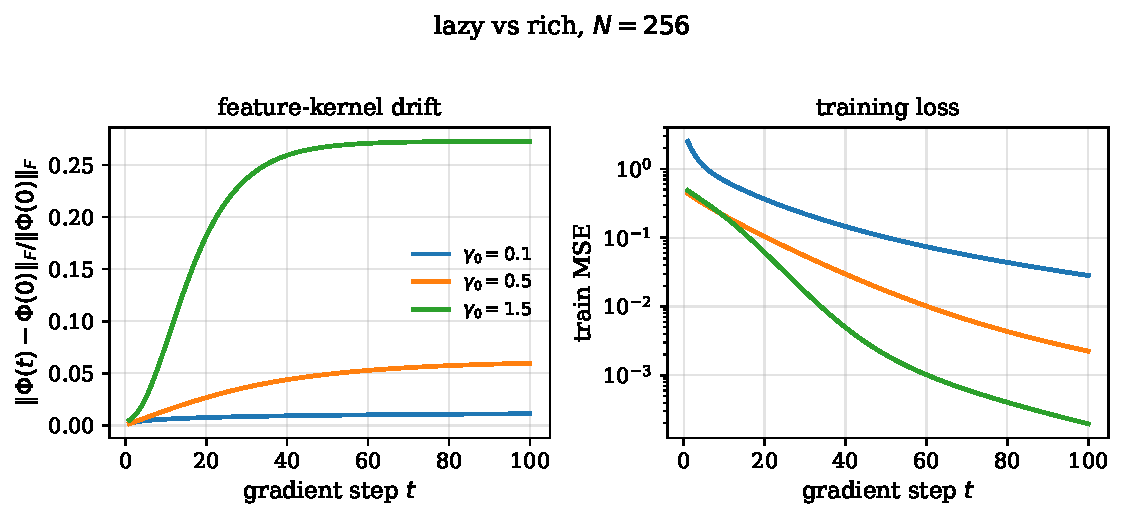
\includegraphics[width=0.95\textwidth]{fig02_lazy_rich.pdf}
\caption{Two-layer ReLU, $N=256$, $\eta=\eta_0\gamma_0^2 N$. Left: relative motion of the hidden feature kernel $\Phi$. Right: training square loss. Only $\gamma_0$ is varied.}
\label{fig:lazy-rich}
\end{figure}

\begin{exercise}
For $f=\gamma_0^{-1}N^{-1/2}v\cdot\ph(Wx/\sqrt{D})$ and $c=0$, compute the $N$-scaling of $\partial_t W$ and $\partial_t v$. Recover $d=\tfrac12$ as the condition that $W$ moves by $\ON{1}$.
\end{exercise}

\section{Infinite-width description}
\label{sec:inf}

\subsection{NNGP recursion}

Fix~\eqref{eq:mup} at initialization. A single first-layer unit is
\begin{equation}
  h^{(1)}_{i}(x)
  =D^{-1/2}\sum_{j=1}^{D} W^{(1)}_{ij}x_j,
  \qquad
  W^{(1)}_{ij}\sim\mathcal{N}(0,1).
  \label{eq:h1}
\end{equation}
The pair $\bigl(h^{(1)}_i(x),h^{(1)}_i(x')\bigr)$ is Gaussian with covariance $\Phi^{(0)}(x,x')=D^{-1}x\cdot x'$, and distinct neurons are independent.

Layer $\ell+1$ is a sum of $N$ i.i.d.\ terms. Because $W^{(\ell+1)}$ is Gaussian,
\begin{equation}
  h^{(\ell+1)}_{i}(\,\cdot\,)
  \;\xrightarrow[N\to\infty]{}\;
  \mathrm{GP}\bigl(0,\,\Phi^{(\ell)}\bigr),
  \qquad
  \Phi^{(\ell)}(x,x')
  =\E\bigl[\ph\bigl(h^{(\ell)}(x)\bigr)\ph\bigl(h^{(\ell)}(x')\bigr)\bigr],
  \label{eq:nngp-rec}
\end{equation}
the expectation being over the GP of layer $\ell$~\cite{neal1996priors,lee2018nngp}. The network output is then a GP with kernel $\Phi^{(L-1)}$. For two inputs the expectation is a two-dimensional Gaussian integral against $\ph$.

\subsection{NTK recursion}

Write $f^{(\ell+1)}=N^{-1/2}W^{(\ell+1)}\ph(h^{(\ell)})$ and $\dot\ph\equiv\ph'$. Differentiating through a layer,
\begin{equation}
  \partial_\theta f^{(\ell+1)}(x)
  =N^{-1/2}\bigl(\partial_\theta W^{(\ell+1)}\bigr)\ph(h^{(\ell)}(x))
  +N^{-1/2}W^{(\ell+1)}\bigl(\dot\ph(h^{(\ell)}(x))\odot \partial_\theta h^{(\ell)}(x)\bigr).
  \label{eq:jac-layer}
\end{equation}
The inner product of two such Jacobians splits into a new-weights term and a previous-layer term. After averaging over $W^{(\ell+1)}\sim\mathcal{N}(0,1)$ and sending $N\to\infty$,
\begin{align}
  \Phi^{(0)}(x,x') &= D^{-1}x\cdot x', \nonumber\\
  \Phi^{(\ell+1)}(x,x') &= \E\bigl[\ph(h)\ph(h')\bigr], \nonumber\\
  \dot\Phi^{(\ell+1)}(x,x') &= \E\bigl[\dot\ph(h)\dot\ph(h')\bigr], \nonumber\\
  \Theta^{(1)}(x,x') &= \Phi^{(0)}(x,x'), \nonumber\\
  \Theta^{(\ell+1)}(x,x')
  &=
  \Phi^{(\ell)}(x,x')
  +\dot\Phi^{(\ell)}(x,x')\,\Theta^{(\ell)}(x,x'),
  \label{eq:ntk-rec}
\end{align}
where $(h,h')$ is the NNGP pair at layer $\ell$~\cite{jacot2018ntk,lee2019wide}. The first term in the last line is the kernel of the incoming activations; the second gates the previous NTK by $\dot\ph$. In NTK scaling ($d=0$), $\Theta(t)=\Theta(0)$ and~\eqref{eq:test-sol} applies with $K=\Theta^{(L)}$.

\subsection{Two-layer DMFT}

Return to~\eqref{eq:mup} with $L=2$:
\begin{equation}
  h_\mu(t)=D^{-1/2}W(t)x_\mu,
  \qquad
  f_\mu(t)=\gamma_0^{-1}N^{-1/2}\,v(t)\cdot\ph\bigl(h_\mu(t)\bigr).
  \label{eq:two-layer}
\end{equation}
Integrating the gradient flow,
\begin{align}
  v(t)&=v(0)+\frac{\eta_0\gamma_0}{P\sqrt{N}}\int_0^t\dd s\sum_{\nu}\Delta_\nu(s)\,\ph\bigl(h_\nu(s)\bigr),
  \label{eq:v-int}\\
  W(t)&=W(0)+\frac{\eta_0\gamma_0}{P\sqrt{D}}\int_0^t\dd s\sum_{\nu}\Delta_\nu(s)\,g_\nu(s)\,x_\nu^\top,
  \label{eq:W-int}
\end{align}
with $g_{\nu,i}\propto v_i\dot\ph(h_{\nu i})$. Substitute into $h_\mu$:
\begin{equation}
  h_\mu(t)
  =\underbrace{D^{-1/2}W(0)x_\mu}_{\chi_\mu(t)}
  +\frac{\eta_0\gamma_0}{P}\int_0^t\dd s\sum_{\nu}
  \Delta_\nu(s)\,G_{\mu\nu}(t,s)\,\Phi^{(0)}_{\mu\nu},
  \label{eq:h-int}
\end{equation}
up to the precise index placement on $\Phi^{(0)}$. The initial field $\chi$ is Gaussian with covariance $\Phi^{(0)}$. The kernels
\begin{equation}
  \Phi_{\mu\nu}(t,s)=N^{-1}\ph(h_\mu(t))\cdot\ph(h_\nu(s)),
  \qquad
  G_{\mu\nu}(t,s)=N^{-1}g_\mu(t)\cdot g_\nu(s)
  \label{eq:dmft-kernels}
\end{equation}
concentrate as $N\to\infty$ on deterministic two-time order parameters~\cite{bordelon2022selfconsistent}. Self-consistency: $\Phi$ and $G$ computed from the process~\eqref{eq:h-int} must reproduce~\eqref{eq:dmft-kernels}.

The integral term in~\eqref{eq:h-int} is proportional to $\gamma_0$. Sending $\gamma_0\to 0$ freezes $h(t)=h(0)$ and recovers
\begin{equation}
  \partial_t f_\mu
  =\frac{\eta_0}{P}\sum_{\nu}\Theta_{\mu\nu}(0)\,\Delta_\nu.
  \label{eq:dmft-lazy}
\end{equation}

For $L>2$ each layer has its own pair $(\Phi^{(\ell)},G^{(\ell)})$, and the preactivations are coupled GPs across time. The closure is still $O(P^2)$ kernels rather than $O(N)$ neurons.

If $\ph(h)=h$, the kernels stay Gaussian and the dynamics reduce to the SVD flow of~\cite{saxe2014exact}: input--output modes train independently, with time constants set by their singular values. Infinite width does not by itself freeze features; a linear network in $\mu$P scaling still moves its internal SVD.

\begin{exercise}
From~\eqref{eq:v-int}--\eqref{eq:W-int}, show that $\gamma_0\to 0$ at fixed $\eta_0$ freezes $W$ while still allowing $v$ to interpolate on an $O(1)$ timescale.
\end{exercise}

\section{Generalization in the lazy regime}
\label{sec:gen}

Once $K$ is frozen, training is kernel ridge~\eqref{eq:ridge}. Three views of the same estimator, following~\cite{hastie2022surprises} and the ridge lectures in APMTH 226.

\subsection{Three views of ridge}

Let $X\in\R^{P\times M}$ be a design (rows $\Phi(x_\mu)^\top$), $y\in\R^{P}$, and
\begin{equation}
  \hat w
  =\argmin_w\ \frac1{2P}\|Xw-y\|^2+\frac\lambda2\|w\|^2
  =\frac1P\Bigl(\frac1P X^\top X+\lambda I\Bigr)^{-1} X^\top y.
  \label{eq:ridge-primal}
\end{equation}
\emph{Interpolation.} If $P>M$ and $\lambda\downarrow 0$, this is ordinary least squares, $\hat w=(X^\top X)^{-1}X^\top y$. If $P<M$, the push-through identity
\begin{equation}
  X^\top(XX^\top+\lambda P I)^{-1}
  =\bigl(X^\top X+\lambda P I\bigr)^{-1}X^\top
  \label{eq:push}
\end{equation}
gives the min-norm interpolant $\hat w=X^\top(XX^\top)^{-1}y$ as $\lambda\downarrow 0$.

\emph{Dynamics.} Gradient flow on square loss starting at $w=0$ converges to that min-norm interpolant. This is~\eqref{eq:lin-gf} in weight space, and~\eqref{eq:ridgeless} in function space.

\emph{Bayes.} Likelihood $y\mid X,w\sim\mathcal{N}(Xw,\sigma^2 I)$ and prior $w\sim\mathcal{N}(0,\sigma_0^2 I)$ have posterior mean equal to~\eqref{eq:ridge-primal} with $\lambda=\sigma^2/\sigma_0^2$.

\subsection{Population eigenbasis}

On $L^2(P_x)$ the kernel has
\begin{equation}
  \int K(x,x')\,\psi_k(x')\,\dd P_x(x')
  =\lambda_k\psi_k(x),
  \qquad
  \lambda_1\ge\lambda_2\ge\cdots\ge 0.
  \label{eq:mercer}
\end{equation}
Expand the target $f^\star(x)=\E[y\mid x]=\sum_k \bar a_k\psi_k$, and write $t_k\equiv\bar a_k^2$. Additive label noise has variance $\sigma^2$.

In the deterministic-equivalence limit~\cite{bordelon2020spectrum,canatar2021spectral,hastie2022surprises} the coefficient of mode $k$ concentrates on
\begin{equation}
  \hat a_k
  =\frac{\lambda_k}{\lambda_k+\kappa}\,\bar a_k
  +\text{(mean-zero sampling noise)},
  \label{eq:mode-shrink}
\end{equation}
where the effective ridge $\kappa$ solves
\begin{equation}
  \kappa=\lambda+\kappa\sum_{k}\frac{\lambda_k}{P(\lambda_k+\kappa)}.
  \label{eq:kappa}
\end{equation}
Ridgeless learning is $\lambda\to 0^+$ with $\kappa$ remaining positive when $P$ does not saturate every mode. Equation~\eqref{eq:kappa} is a self-consistent accounting of the degrees of freedom absorbed by the sample: each mode contributes a factor $\lambda_k/(\lambda_k+\kappa)$, and $\kappa$ is whatever is left of $\lambda$ after that absorption.

\subsection{Bias, variance, learning curve}

Square-loss population risk then decomposes as
\begin{equation}
  R
  =\sum_k t_k\Bigl(\frac{\kappa}{\lambda_k+\kappa}\Bigr)^2
  +\frac{\sigma^2}{P}\sum_k\Bigl(\frac{\lambda_k}{\lambda_k+\kappa}\Bigr)^2
  +\sigma^2.
  \label{eq:R-spectral}
\end{equation}
The first sum is bias: mode $k$ is learned once $P\lambda_k\gtrsim\kappa$. The second is variance from fitting noise.

If $\lambda_k$ decays, as it does for NTK, Laplace, and ReLU kernels on the sphere, small-$k$ modes reach $\lambda_k\gg\kappa/P$ first. The residual of mode $k$ falls only once $P\gtrsim\kappa/\lambda_k$: \emph{spectral bias}. For fixed $\{\lambda_k\}$, a target with $t_k$ on large-$\lambda_k$ modes has smaller $R$ at given $P$: \emph{task--model alignment}~\cite{canatar2021spectral}. As $\lambda\to 0$ and $P$ crosses the rank of $\hat K$, the variance term spikes (\emph{double descent}); a decaying spectrum or $\lambda>0$ smooths the spike~\cite{belkin2019reconciling,hastie2022surprises}.

\begin{figure}[ht]
\centering
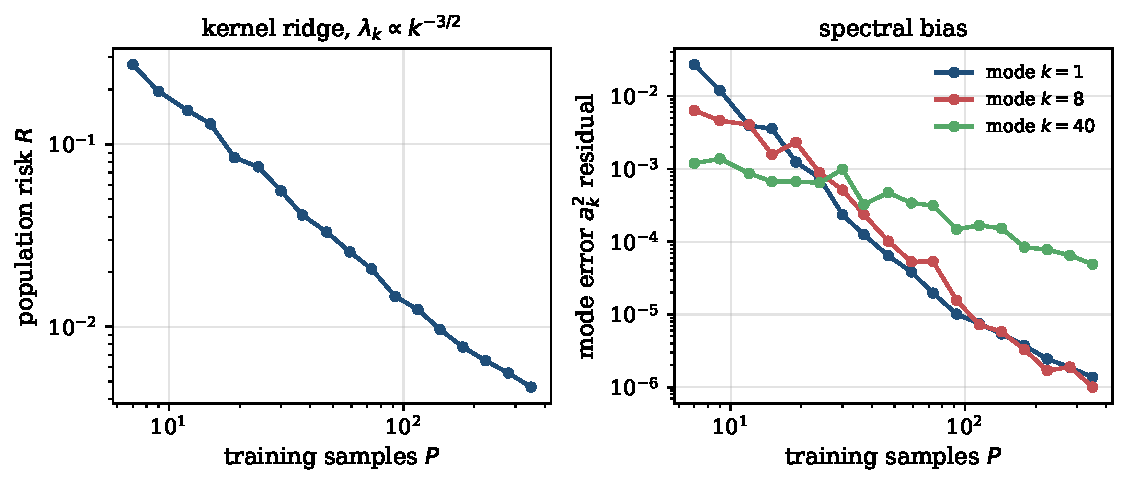
\includegraphics[width=0.95\textwidth]{fig05_kernel_learning.pdf}
\caption{Kernel ridge with $\lambda=10^{-3}$ and $\lambda_k\propto k^{-3/2}$. Left: population risk versus $P$. Right: residual power in modes $k=1,8,40$. Averages over Gaussian designs.}
\label{fig:learn}
\end{figure}

Lazy neural generalization is~\eqref{eq:R-spectral} for the NTK spectrum $\Theta^{(L)}(t=0)$. On the sphere that spectrum is a Gegenbauer transform~\cite{canatar2021spectral}.

\begin{exercise}
From~\eqref{eq:kappa}, with $\sigma=0$ and $\lambda_k=k^{-\beta}$, $\beta>1$, estimate the $P$ at which mode $k$ is half-learned ($\kappa\approx\lambda_k$).
\end{exercise}

\section{Effective theory at initialization}
\label{sec:crit}

The infinite-width kernels still depend on depth through a nonlinear map. That map can explode, vanish, or sit at a fixed point, according to the initialization variances~\cite{poole2016exponential,schoenholz2017deep,roberts2022pdlt}. Finite-width corrections around the fixed point are organized in $L/N$.

\subsection{Gaussian integrals}

If $z\sim\mathcal{N}(0,K)$ in $\R^{m}$,
\begin{equation}
  \E\bigl[e^{j\cdot z}\bigr]
  =\exp\bigl(\tfrac12 j^\top K j\bigr).
  \label{eq:gauss-gen}
\end{equation}
Odd moments vanish, and
\begin{equation}
  \E[z_{a}z_{b}]=K_{ab},
  \qquad
  \E[z_{a}z_{b}z_{c}z_{d}]
  =K_{ab}K_{cd}+K_{ac}K_{bd}+K_{ad}K_{bc}.
  \label{eq:wick}
\end{equation}
For a general activation,
\begin{equation}
  \E\bigl[\ph(h)\ph(h')\bigr]
  =\int\frac{\dd u\,\dd v}{2\pi\sqrt{\det C}}\,
  \ph(u)\ph(v)\,
  \exp\bigl(-\tfrac12 (u,v)\,C^{-1}(u,v)^\top\bigr),
  \label{eq:2d-gauss}
\end{equation}
with $C=\bigl(\begin{smallmatrix}K_{xx}&K_{xx'}\\ K_{xx'}&K_{x'x'}\end{smallmatrix}\bigr)$.

\subsection{Kernel recursion}

Biases $b_i\sim\mathcal{N}(0,C_b)$ and rescaled weight variance $C_W$ give
\begin{equation}
  K^{(\ell+1)}_{\alpha\beta}
  =C_b+C_W\,\E\bigl[\ph(z_\alpha)\ph(z_\beta)\bigr]_{K^{(\ell)}},
  \qquad
  K^{(1)}_{\alpha\beta}
  =C_b+C_W\,D^{-1}x_\alpha\cdot x_\beta.
  \label{eq:K-rec}
\end{equation}
On the diagonal, $q_\ell\equiv K^{(\ell)}(x,x)$ is a 1d map $q\mapsto F(q)$. Off the diagonal one tracks $c_\ell=K^{(\ell)}(x,x')/\sqrt{q_\ell(x)q_\ell(x')}$.

Linearizing about a fixed point $q_\star=F(q_\star)$,
\begin{equation}
  \chi
  \equiv
  F'(q_\star)
  =C_W\,\E\bigl[\dot\ph(z)^2\bigr]_{z\sim\mathcal{N}(0,q_\star)}.
  \label{eq:chi}
\end{equation}
Then $\delta q_{\ell+1}=\chi\,\delta q_\ell+\cdots$, and the off-diagonal perturbation $\delta c$ is multiplied by the same $\chi$. Hence $\chi<1$ is ordered (signals vanish), $\chi>1$ is chaotic (signals explode), and $\chi=1$ is critical. The pair $(\chi=1,\,q_\star=F(q_\star))$ fixes $(C_W,C_b)$ for a given $\ph$.

\paragraph{Deep linear.}
$\ph(z)=z$ implies $K^{(\ell+1)}=C_W K^{(\ell)}$, so $K^{(\ell)}=C_W^{\ell-1}K^{(1)}$. Criticality is $C_W=1$; any other choice explodes or vanishes exponentially in depth.

\paragraph{tanh.}
Odd, $\dot\ph(0)=1$. At $C_b=0$ the origin $q_\star=0$ is a fixed point and $\chi(0)=C_W$. Criticality at the origin is $C_W=1$. For $C_W<1$ the kernel collapses with depth; for $C_W>1$ it grows until the nonlinearity saturates. The same pattern holds for $\sin$ and $\mathrm{erf}$ (the $K'=0$ class of~\cite{roberts2022pdlt}).

\paragraph{ReLU.}
Homogeneous. The Cho--Saul formula~\eqref{eq:cho-saul} is the diagonal-plus-cosine map. Criticality is $C_W=2$ at $C_b=0$ (He initialization). There is no exponentially stable $q_\star>0$ at $C_b=0$ other than this ray.

\begin{figure}[ht]
\centering
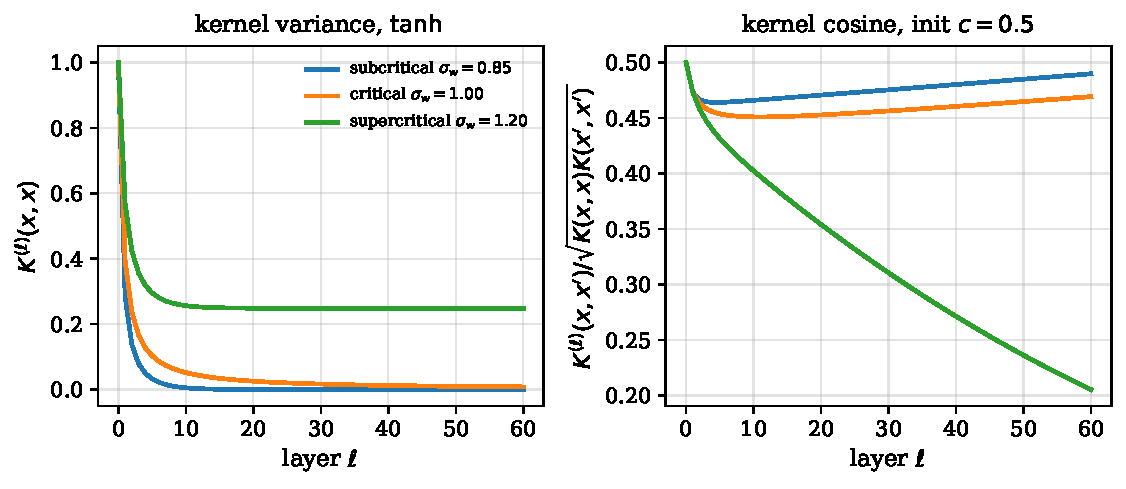
\includegraphics[width=0.95\textwidth]{fig03_criticality.pdf}
\caption{$\tanh$ kernel recursion~\eqref{eq:K-rec} with $C_b=0$. Left: $K^{(\ell)}(x,x)$. Right: cosine of two inputs, initialized at $c=0.5$. Subcritical, critical ($C_W=1$), and supercritical $C_W$.}
\label{fig:crit}
\end{figure}

\subsection{\texorpdfstring{Four-point functions and $L/N$}{Four-point functions and L/N}}

At finite $N$ the empirical metric
\begin{equation}
  G_{\alpha\beta}
  \equiv
  N^{-1}\sum_{i=1}^{N} h_{i}(x_\alpha)h_{i}(x_\beta)
  \label{eq:metric}
\end{equation}
fluctuates about $K_{\alpha\beta}$. For a \emph{deep linear} net, a single input, $C_b=0$ and $C_W=1$, Wick's theorem on $z_i=\sum_j N^{-1/2}W_{ij}h_j$ gives the recursion
\begin{equation}
  \E[G]
  =K,
  \qquad
  \Var(G^{(\ell+1)})
  =\Var(G^{(\ell)})+\frac{2K^2}{N}.
  \label{eq:var-rec}
\end{equation}
Iterating from a deterministic first layer,
\begin{equation}
  \Var\bigl(G^{(L)}\bigr)
  =\frac{2K^2 L}{N}.
  \label{eq:LN}
\end{equation}
The same $L/N$ appears for nonlinear $\ph$ at criticality, with a different $O(1)$ prefactor $V_0(\ph)$~\cite{roberts2022pdlt}. Infinite-width formulae are accurate when $L/N\ll 1$; $1/N$ corrections accumulate additively over depth.

\begin{figure}[ht]
\centering
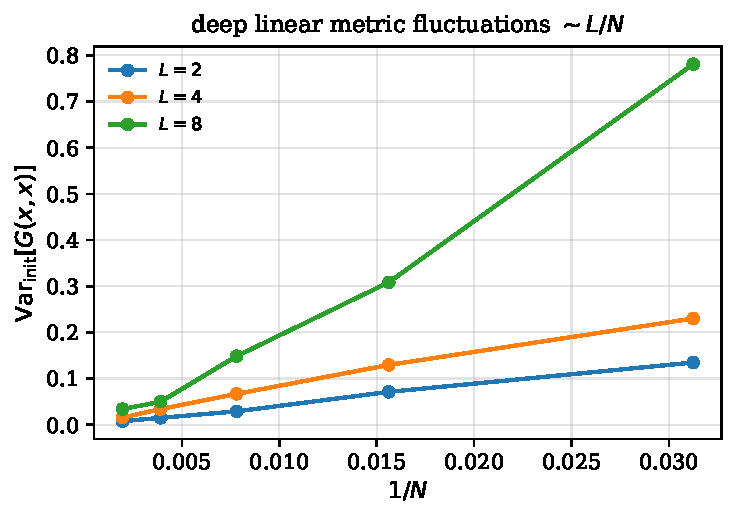
\includegraphics[width=0.72\textwidth]{fig04_finite_width.pdf}
\caption{Deep linear MLPs at $C_W=1$. Variance of $G(x,x)=N^{-1}\|h^{(L)}(x)\|^2$ across $400$ initializations, versus $1/N$, for depths $L=2,4,8$.}
\label{fig:fn}
\end{figure}

\begin{exercise}
Derive~\eqref{eq:var-rec} from~\eqref{eq:wick} for $z=N^{-1/2}Wh$ with $W_{ij}\sim\mathcal{N}(0,1)$ independent of $h$.
\end{exercise}

\section{Finite-width representation learning}
\label{sec:dntk}

Infinite-width NTK dynamics are linear in function space: $f(t)$ stays in the affine space $f(0)+\mathrm{span}\{K(x_\mu,\,\cdot\,)\}$. The first correction that moves the kernel is $O(L/N)$ at criticality~\cite{roberts2022pdlt} and $O(\gamma_0)$ at infinite width in $\mu$P.

\subsection{Quadratic model}

Taylor-expand in $\delta\theta=\theta-\theta_0$:
\begin{equation}
  f(x;\theta_0+\delta\theta)
  =f(x;\theta_0)
  +J(x)\cdot\delta\theta
  +\tfrac12\,\delta\theta^\top H(x)\,\delta\theta
  +O(\|\delta\theta\|^3),
  \label{eq:taylor}
\end{equation}
with $J(x)=\partial_\theta f(x)|_{\theta_0}$ and $H_{pq}(x)=\partial_{\theta_p}\partial_{\theta_q}f(x)|_{\theta_0}$. The first two terms are a linear model with features $J$; their Gram matrix is the NTK
\begin{equation}
  \Theta(x,x')=J(x)\cdot J(x').
  \label{eq:ntk-again}
\end{equation}
Truncating at linear order in $\delta\theta$ recovers frozen-NTK training. The quadratic term is the leading representation-learning correction.

\subsection{Differential of the NTK}

Along a parameter direction $u$,
\begin{equation}
  \bigl(\nabla_u\Theta\bigr)(x,x')
  =H(x)\,u\cdot J(x')
  +J(x)\cdot H(x')\,u.
  \label{eq:dntk}
\end{equation}
The trilinear kernel
\begin{equation}
  D(x,x',x'')
  \equiv
  \partial_\theta\Theta(x,x')\cdot\partial_\theta f(x'')
  \label{eq:dntk-def}
\end{equation}
is the dNTK~\cite{roberts2022pdlt}. It vanishes for a linear model ($H=0$). In NTK scaling $\delta\theta=O(N^{-1/2})$, so $D$ does not move $\Theta$ by an $O(1)$ amount. At finite $N$, one GD step of size $\eta$ updates the kernel by
\begin{equation}
  \Delta\Theta(x,x')
  =-\frac{\eta}{P}\sum_{\mu} D(x,x',x_\mu)\,\Delta_\mu
  +O(\eta^2).
  \label{eq:dtheta}
\end{equation}

The first layer of an MLP contributes $D^{(1)}=0$ (the map $x\mapsto W^{(1)}x$ is linear in $W^{(1)}$). Each subsequent layer sources a nonzero $D$ from $\ddot\ph$ and from products of earlier $\Theta$'s. After $L$ layers at criticality, $D=O(L)$, hence
\begin{equation}
  \frac{\Delta\Theta}{\Theta}
  =O\!\left(\frac{L}{N}\right)
  \label{eq:dtheta-LN}
\end{equation}
for NTK-scaled GD with $\eta=O(1)$. The same ratio is $O(1)$ in $\mu$P at infinite $N$.

\subsection{Nearly-kernel prediction}

Keeping the quadratic term in~\eqref{eq:taylor} and going to a stationary point of square loss, the trained predictor is, to first order in $D$,
\begin{equation}
  f(x;\infty)
  =f_{\mathrm{NTK}}(x)
  +\frac1{2P^2}\sum_{\mu\nu}
  D(x,x_\mu,x_\nu)\,c_{\mu\nu}
  +O\bigl((L/N)^2\bigr),
  \label{eq:nearly-kernel}
\end{equation}
where $c_{\mu\nu}$ is bilinear in the training residuals of the linear problem~\cite{roberts2022pdlt}. Predictions are still determined by a finite collection of kernels $(\Theta,D)$.

The kernel picture is accurate when $L/N\ll 1$ and $d<\tfrac12$. Representation learning is $O(1)$ when $L/N=O(1)$, or when $d=\tfrac12$ with $\gamma_0=O(1)$. At fixed compute the useful aspect ratio is an $O(1)$ value of $L/N$: large enough that $D$ can move features, small enough that the $L/N$ expansion remains under control.

\begin{exercise}
For $f(x)=\tfrac12 A x^2$ with scalar $x$ and parameter $A$, compute $\Theta$ and $D$, and verify~\eqref{eq:dtheta} for one GD step.
\end{exercise}


\appendix
\section{Definitions}

\begin{description}[style=nextline,leftmargin=1.1em,itemsep=0.55em,font=\normalfont\bfseries]

\item[Gram matrix.]
For vectors $v_1,\ldots,v_P$, the matrix $G_{\mu\nu}=v_\mu\cdot v_\nu$. Always positive semidefinite. The kernel matrix $\hat K_{\mu\nu}=K(x_\mu,x_\nu)$ is the Gram matrix of the feature maps $\Phi(x_\mu)$.

\item[Positive-definite kernel.]
A symmetric $K:\mathcal{X}\times\mathcal{X}\to\R$ such that $\sum_{\mu\nu}c_\mu c_\nu K(x_\mu,x_\nu)\ge 0$ for all finite collections $\{x_\mu\}$ and all $c\in\R^{P}$. Equivalent, by Mercer, to $K(x,x')=\Phi(x)\cdot\Phi(x')$ for some (possibly infinite-dimensional) feature map $\Phi$.

\item[Feature map / kernel trick.]
A lift $\Phi:\mathcal{X}\to\mathcal{H}$ into a Hilbert space. Inner products in $\mathcal{H}$ can be evaluated as $K(x,x')$ without writing $\Phi$ down. The SVM dual~\eqref{eq:svm-dual} and kernel ridge~\eqref{eq:ridge} depend on data only through $K$.

\item[RKHS.]
The reproducing kernel Hilbert space $\mathcal{H}_K$ of a kernel $K$ is the completion of $\mathrm{span}\{K(x,\,\cdot\,):x\in\mathcal{X}\}$ under the inner product $\langle K(x,\,\cdot\,),K(x',\,\cdot\,)\rangle_{\mathcal{H}_K}=K(x,x')$. Evaluation is continuous: $h(x)=\langle h,K(x,\,\cdot\,)\rangle_{\mathcal{H}_K}$.

\item[Representer theorem.]
Empirical-risk minimizers in $\mathcal{H}_K$ with an RKHS-norm penalty lie in $\mathrm{span}\{K(x_\mu,\,\cdot\,)\}_{\mu=1}^{P}$. The infinite-dimensional problem collapses to $P$ coefficients.

\item[Support vector.]
A training point with nonzero dual coefficient $\alpha_\mu$ in~\eqref{eq:kkt}. Complementary slackness puts it on the margin. The max-margin hyperplane is a linear combination of support vectors only.

\item[Cho--Saul formula.]
The kernel of a random ReLU feature $\ph(z)=\max(z,0)$. For $w\sim\mathcal{N}(0,D^{-1}I)$ and $\vartheta=\arccos\bigl(x\cdot x'/(\|x\|\|x'\|)\bigr)$,
\[
  \E\bigl[\ph(w\cdot x)\ph(w\cdot x')\bigr]
  =\frac{\|x\|\|x'\|}{2\pi D}\bigl(\sin\vartheta+(\pi-\vartheta)\cos\vartheta\bigr).
\]
This is~\eqref{eq:cho-saul}. The NNGP recursion for deep ReLU nets is the iteration of this map.

\item[Gradient flow.]
The ODE $\dot\theta=-\eta\nabla_\theta\loss(\theta)$, the $\eta\to 0$ limit of gradient descent. In these notes, the source of all training dynamics.

\item[Gaussian process.]
A random function $f$ such that $\bigl(f(x_1),\ldots,f(x_n)\bigr)$ is jointly Gaussian for every finite set. Specified by a mean and a covariance kernel $K(x,x')=\E[f(x)f(x')]$. An infinite-width net at initialization is a GP with the NNGP kernel.

\item[NNGP.]
Neural network Gaussian process: the $N\to\infty$ law of $f(\,\cdot\,;\theta)$ at initialization. Covariance given by the feature-kernel recursion~\eqref{eq:nngp-rec}.

\item[Neural tangent kernel.]
$K(x,x';t)=\partial_\theta f(x;t)\cdot\partial_\theta f(x';t)$. The metric that makes gradient flow on $\theta$ into an ODE on functions~\eqref{eq:fn-ode}. Frozen if features do not move.

\item[Trilinear kernel.]
A scalar $T(x,x',x'')$ linear in each slot. The dNTK $D(x,x',x'')=\partial_\theta\Theta(x,x')\cdot\partial_\theta f(x'')$ is trilinear in the Jacobians and Hessians of $f$: it contracts $H(x)$, $J(x')$, and $J(x'')$.

\item[Order parameter.]
A macroscopic summary (here $\Phi$, $G$, $K$, $\Theta$) that concentrates as $N\to\infty$. The microscopic weights fluctuate; the order parameters obey a closed equation.

\item[NTK parameterization / $\mu$P.]
Two scalings of~\eqref{eq:pb-mlp} with width. NTK parameterization: $d=0$, features freeze, $K(t)=K(0)$. Maximal update parameterization ($\mu$P) / mean-field: $d=\tfrac12$, features move by $\ON{1}$, kernels obey DMFT. See~\eqref{eq:mup}.

\item[DMFT.]
Dynamical mean-field theory. After $N\to\infty$, each neuron is an independent copy of a stochastic process whose statistics $(\Phi,G)$ are determined self-consistently from that same process. Replaces $O(N)$ coupled ODEs by $O(P^2)$ kernel equations.

\item[Criticality.]
Initialization $(C_W,C_b)$ at which the kernel recursion has $\chi=F'(q_\star)=1$. Signals neither explode nor vanish with depth. For $\tanh$ at $C_b=0$, $C_W=1$; for ReLU, $C_W=2$.

\item[Stability parameter $\chi$.]
$\chi=C_W\E[\dot\ph(z)^2]$ at the kernel fixed point. Multiplies perturbations of $K$ from layer to layer. $\chi=1$ is critical.

\item[Depth-to-width ratio.]
$L/N$. Leading finite-width expansion parameter at criticality: $\Var(G)\sim (L/N)V_0$. Kernel formulae hold for $L/N\ll 1$; dNTK representation learning is $O(L/N)$.

\item[dNTK.]
Differential of the NTK, $D(x,x',x'')=\partial_\theta\Theta(x,x')\cdot\partial_\theta f(x'')$. Trilinear kernel that sources $\dot\Theta$ at finite width. Vanishes for linear models and, to leading order, in infinite-width NTK scaling.

\item[Wick's theorem.]
Gaussian moment factorization: $\E[z_{a_1}\cdots z_{a_{2n}}]$ is the sum over pairings of products of covariances. Used to close four-point recursions for deep linear nets,~\eqref{eq:var-rec}.

\item[Deterministic equivalence.]
In high dimension, a random matrix functional (here the ridge resolvent $(\hat\Sigma+\lambda I)^{-1}$) concentrates on a non-random proxy, typically involving an effective ridge $\kappa$. Converts the random learning curve into~\eqref{eq:R-spectral}.

\item[Spectral bias.]
Kernel machines learn eigenmodes of $K$ in decreasing order of $\lambda_k$. Mode $k$ is fit once $P\lambda_k\gtrsim\kappa$.

\item[Lazy / rich training.]
Lazy: $K(t)\approx K(0)$, the net is a linear model in its initial Jacobian features. Rich: hidden features $\Phi(t)$ move by $\ON{1}$. Selected by $d$ in~\eqref{eq:lr-scale}, or by $\gamma_0$ at finite $N$.

\end{description}


\bibliographystyle{plain}
\bibliography{refs}

\end{document}
